%---------------------------------------------
%	7. Application & Perform of GNN Algorithm
%---------------------------------------------

\chapter{Application to the TrackML Model, Results and Discussion}
\label{chapter-7}


Application of the GNN algorithm to the TrackML detector data, the endcap and barrel region.

Section ... presents the results of the application of the GNN algorithm on the endcap region and Section ... discusses an outlook onto ....

%  The preliminary results related to track reconstruction efficiency and purity metrics are presented and discussed.
%The main results we get from application of this algorithm, the track reconstruction efficiency, the purity metrics, computational performance. Comparison with other algorithms.



\section{Endcap Results and Performance Evaluation}

% track purity, particle purity, track reconstruction efficiency
% TODO: mention here that the parabolic track state model was used and the joint track state was used, and mention the section here

%nips-2018-competation
%Data.
%We used the fast (10s per event) and accurate simulation engine ACTS4 [6] to generate the challenge data. It allowed us to generate realistic data emulating a full Silicon LHC detector (see Fig 3), while providing us with the ground truth of particle trajectory membership. Thus, for each event we obtained the “detected” 3D points coordinates (and additional features), and, as ground truth, the list of points associated to each track. There is a one to one relationship between the true 3D points and the reconstructed ones.

%\begin{itemize}
%    \item Application on TrackML model, endcap volume only, metrics, performance eval etc, track reconstruction efficiency, track purity and particle purity, comparison with TrackML solutions
%    \item Track reconstruction efficiency, track purity, particle purity
%    \item Performance Evaluation
%    \item execution time?
%\end{itemize}

% need to present the average over many events here


\section{Outlook}
\subsection{Extension to the Barrel Region}
\subsection{Software Optimisations}

\subsection{Other Approaches}
\subsubsection{Community Detection}

%If a subgraph does not meet the criteria to qualify as a good track candidate, a \textit{Community Detection} algorithm \cite{community} is applied in order to further partition the set of nodes. Community Detection is a generalisation of CCA and works by using a distance metric, typically modularity, in order to label nodes as \textit{closely connected}. Modularity is a benefit function that measures the strength of a particular division of a network using the number of edges. A popular modularity maximisation approach is the Louvain method \cite{python_louvain}, which iteratively optimises local communities until global modularity can no longer be improved. An example illustration of a network partition via Community Detection is shown in Figure \ref{fig:community-detection}. Any subgraphs with zero extracted candidates through this procedure are propagated to further stages for additional processing.

%Community Detection: divides nodes into various clusters based on edge structure. It learns from edge weights, and distance and graph objects similarly. 

%\begin{figure}[htbp]
%    \centering
%    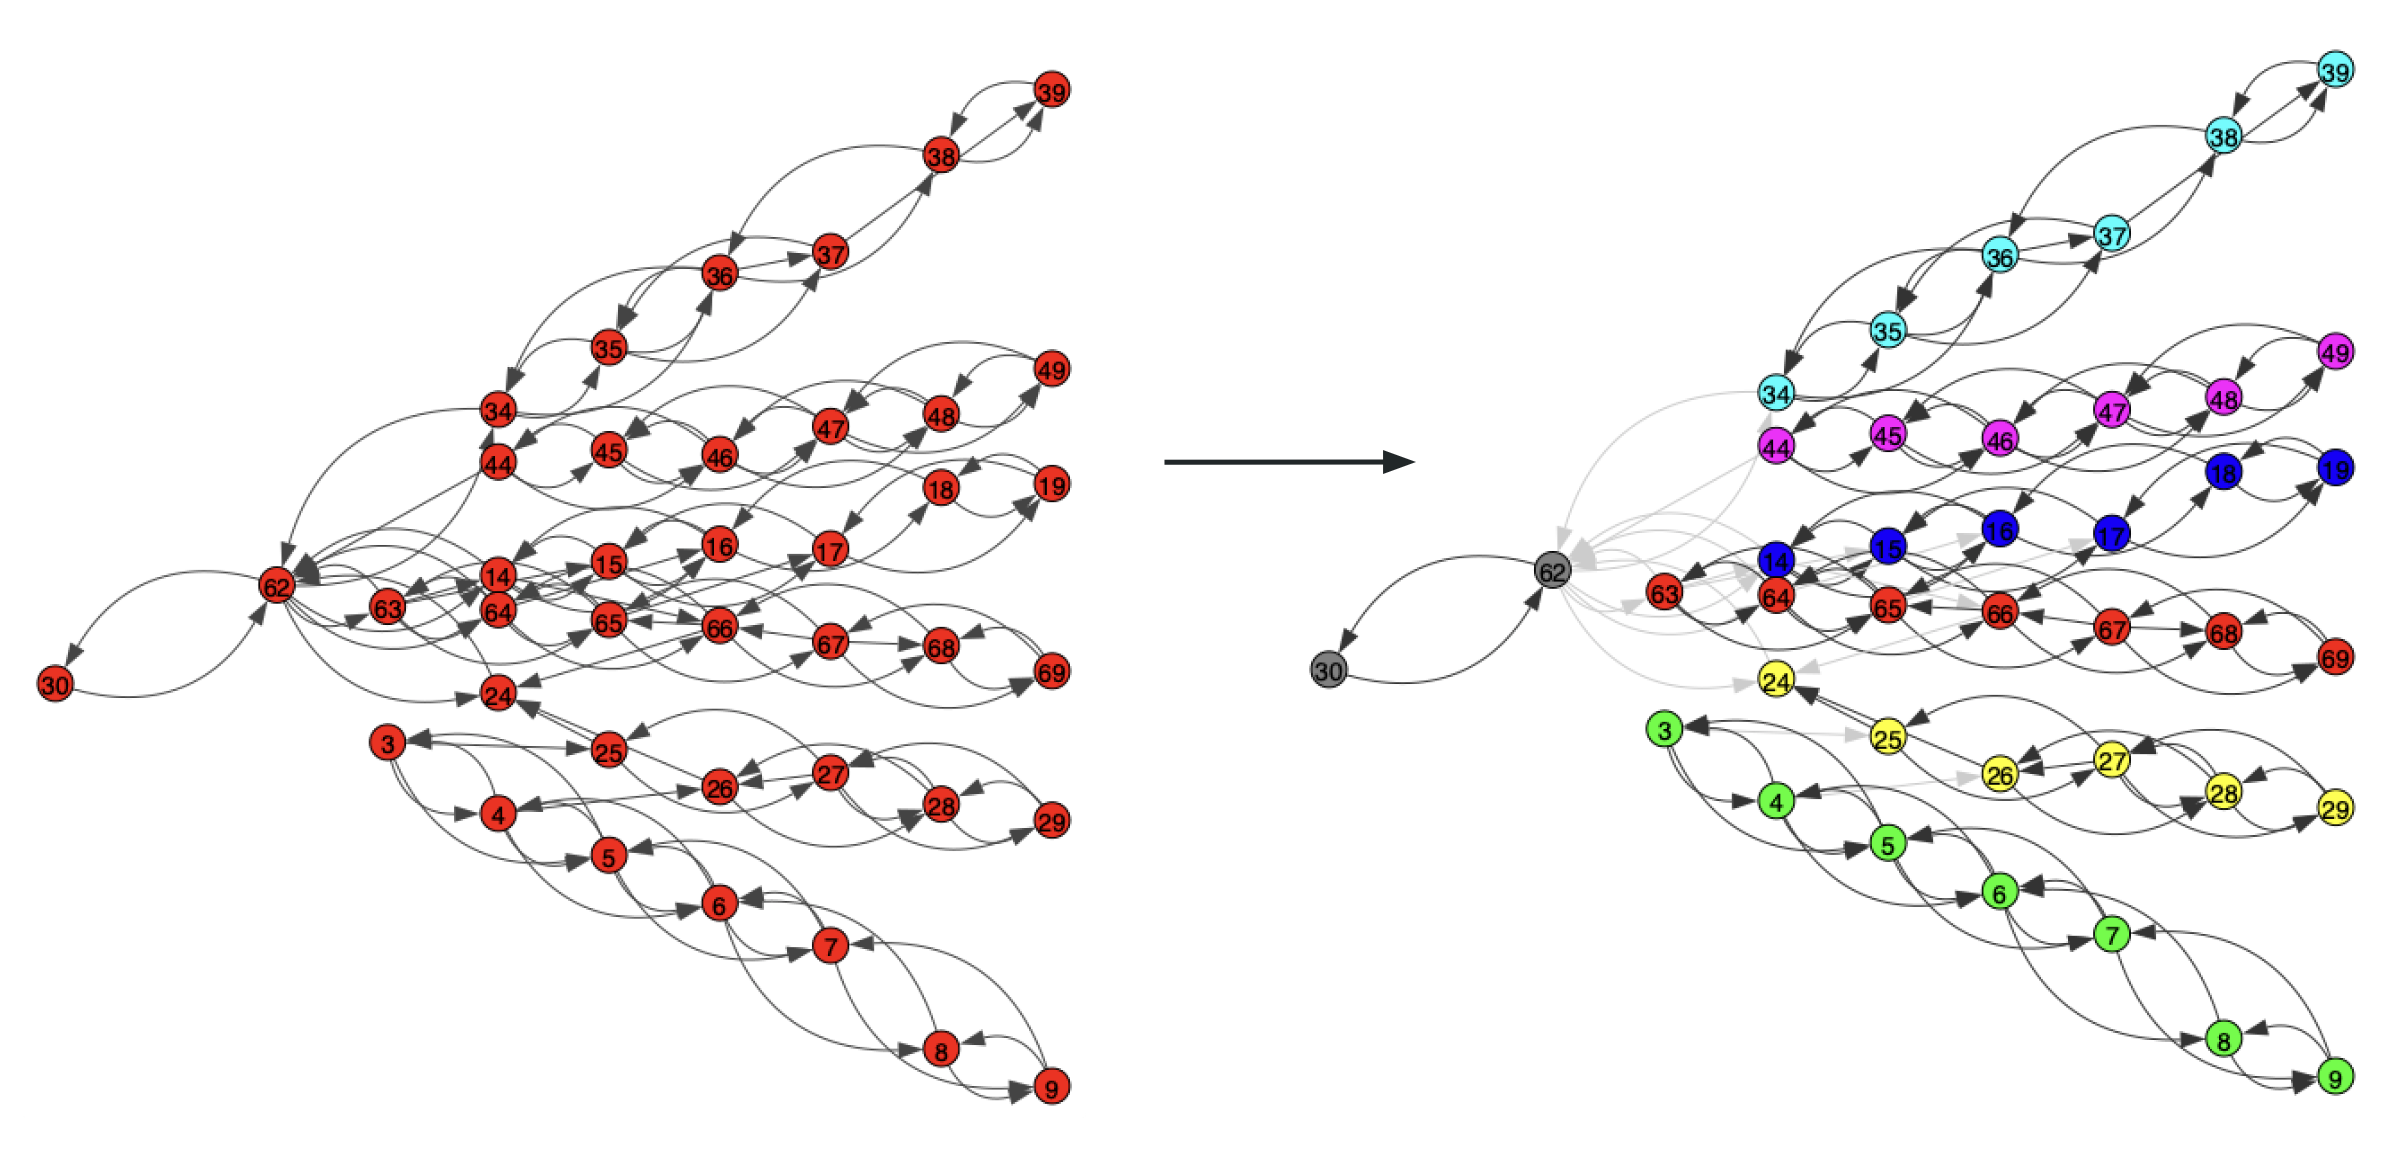
\includegraphics[width=0.98\textwidth]{images/5-gnn-algorithm/community-detection.png}
%    \caption{TODO: caption ....}
%    \label{fig:community-detection}%
%\end{figure}

%\begin{itemize}
%    \item extension to barrel, analysis of results, performance  evaluation, challenges and outlook
%    \item Optimisation - GPU acceleration etc
%\end{itemize}


\section{Conclusions}

% Utilizing message passing to iteratively learn neighbourhood information aids in the pruning of outlier edges within complex regions.

% This key feature of the GNN-based algorithm suggests that the excitation and inhibition rules of individual GNN nodes are designed in such a way to facilitate the “simple-to-complex” approach for “nodes-to-tracks” association. 